%% LaTeX_Thesis_Template.tex
% An unofficial LaTeX template for Cranfield theses.
% 2017/08/14 Daniel Auger's unofficial Cranfield thesis .sty file
% 2023/05/31 Updated by Shaun Forth (SAF) for logo inclusion
% 2023/06/08 SAF removed capitalisation on title pages on advice of Amy 
% Greenaway and Alison Waters. Added Daniel Auger's headers with 
% chapter and section names.
% 2023/06/08 SAF simplified logo inclusion

%%
% This document is an example of the use of the unofficial "cranfieldthesis" 
% LaTeX style file.  I hope it's useful, and a good likeness of the Word template.

\documentclass[12pt,oneside]{book} % for one-sided printing
%\documentclass[12pt,twoside]{book} % for two-sided printing

% Use the custom "cranfieldthesis" LaTeX style file. 
\usepackage{cranfieldthesis}
\usepackage{lscape} % for landscape pages
\usepackage{amsmath}
\usepackage{enumitem}
\usepackage{changepage}
\usepackage{pdfpages}
\usepackage{blindtext}% Just used so we can generate some example text
\usepackage{algorithm}
\usepackage{algpseudocode}
\usepackage{amssymb}
\usepackage{mathtools}
\usepackage[export]{adjustbox}
\usepackage{lipsum}
\usepackage{booktabs}  % For better quality tables
\usepackage{siunitx}
\usepackage{float}
\usepackage{longtable} % Pour les tableaux sur plusieurs pages
\usepackage{tabularx}  % for the X column type
\usepackage{listings}
\usepackage{xcolor}
\usepackage{caption}
\usepackage{xfrac}
\usepackage{indentfirst}
\usepackage{subcaption}
\usepackage{graphicx}
\usepackage{geometry}
\usepackage{titlesec}
\geometry{a4paper, margin=1in}
\hypersetup{
    colorlinks,
    linkcolor={blue!50!blue},
    citecolor={blue!50!blue},
    urlcolor={blue!80!blue}
}

% By default, LaTeX uses a serif font - these are traditionally thought to be
% easier to read.   If you'd prefer sans-serif, please uncomment the 
% following line.
% \renewcommand{\familydefault}{\sfdefault}

% Example parameters for a typical taught MSc course
\title{Future Position Prediction for Pressure Refuelling Port
    of Commercial Aircraft}
\author{Alexis Balayre}
\date{May 2024}
\school{\SATM}
\course{Computational and Software Techniques in Engineering}
\degree{MSc}
\academicyear{2023--2024}
\setCUPartnerLogo{logo-airbus.png}
\supervisors{Dr Boyu Kuang and Dr Stuart Barnes}
\copyrightyear{2024}

% References
% Cranfield Numbered Style
\usepackage[numbers]{natbib} % for nice referencing
\makeatletter % Reference list option change to number and period
\renewcommand\@biblabel[1]{#1.} % from [1] to 1
\makeatother %

\begin{document}

%% Front matter
%
% This is where we do the title page, etc.
%

\frontmatter

% Standard-Form Title Pages
\maketitle

% Abstract and Keywords
\begin{abstract}
    Replace with your abstract text of not more than 300 words.
\end{abstract}

\begin{keywords}
    Replace with at least 6, semicolon seperated keywords (not contained within the thesis title) – this makes the thesis searchable.
\end{keywords}

% Acknowledgements
\chapter{Acknowledgements}
The author would like to thank \dots

% Use single spacing for Table of Contents, List of Figures, etc
{
    \clearpage

    % Table of Contents
    \singlespacing{
        \tableofcontents
    }
    \clearpage

    % List of Figures
    \listoffigures

    \clearpage
    % List of Tables
    \listoftables
}

% The list of abbreviations can't be automatically generated so you need to populate it yourself
\begin{listofabbreviations}
    \abbrev{ML}{Machine Learning}
    \abbrev{DL}{Deep Learning}
    \abbrev{AI}{Artificial Intelligence}
    \abbrev{CNN}{Convolutional Neural Network}
    \abbrev{RNN}{Recurrent Neural Network}
    \abbrev{LSTM}{Long Short-Term Memory}
    \abbrev{GRU}{Gated Recurrent Unit}
    \abbrev{EKF}{Extended Kalman Filter}
    \abbrev{AAGR}{Autonomous Aircraft Ground Refueling}
    \abbrev{AGR}{Aircraft Ground Refueling}
    \abbrev{UAV}{Unmanned Aerial Vehicle}
    \abbrev{AAR}{Autonomous Aerial Refueling}
    \abbrev{DGPS}{Differential Global Positioning System}
    \abbrev{SVM}{Support Vector Machine}
    \abbrev{HOG}{Histogram of Oriented Gradients}
    \abbrev{SOTA}{State-of-the-Art}
    \abbrev{AIS}{Automatic Identification System}
    \abbrev{GPS}{Global Positioning System}
\end{listofabbreviations}

%% Main Matter
%
% This is where we include the main thesis content.
%
\mainmatter\pagestyle{fancy}
\fancyhead[L]{\nouppercase{\leftmark}}
\fancyhead[R]{\nouppercase{\rightmark}}

%%%%%%%%%%%%%%%%%%%%%%%%%%%%%%%%%%%%%%%%%%%%%%%%%%%%%%%%%%%%%%%%%%%%%%%%%%%%%%%%
%%%%%%%%%%%%%%%%%%%%%%%%%%%%%%%%% INTRODUCTION %%%%%%%%%%%%%%%%%%%%%%%%%%%%%%%%%
\chapter{Introduction}
Ground pressure refuelling is a standard method used to refuel commercial
aircraft safely and efficiently. This process involves using a hydrant system,
which consists of underground fuel pipelines connected to a network of fuel
hydrants located at aircraft parking positions~\cite{blakey2011aviation}. The
hydrant system is supplied with fuel from storage tanks, typically located near
the airport~\cite{kazda2015airport}.

When an aircraft is ready for refueling, a hydrant dispenser vehicle, also
known as a hydrant truck or cart, is connected to the hydrant pit using a
flexible hose~\cite{sati2019aircraft}. The hydrant dispenser vehicle is
equipped with a pressure control valve, a flow meter, and a filtration system
to ensure that the fuel meets the required quality
standards~\cite{iata2019guidance}.

The refueling process begins by connecting the hydrant dispenser vehicle to the
aircraft's fuel panel using another flexible hose~\cite{sati2019aircraft}. The
pressure control valve on the hydrant dispenser vehicle is then used to
regulate the fuel pressure and flow rate, ensuring that the fuel is delivered
to the aircraft at the appropriate pressure and volume~\cite{iata2019guidance}.

One of the main advantages of pressure ground refueling is its efficiency. This
method allows for high fuel flow rates, which can significantly reduce aircraft
turnaround times~\cite{blakey2011aviation}. Additionally, the use of
underground pipelines eliminates the need for fuel trucks, reducing traffic
congestion and the risk of accidents on the apron~\cite{kazda2015airport}.

Safety is another critical aspect of pressure ground refueling. The hydrant
system is designed with multiple safety features, such as emergency shutdown
valves and leak detection systems, to minimise the risk of fuel spills and
fires~\cite{iata2019guidance}. Moreover, the hydrant dispenser vehicles are
equipped with safety devices, such as dead man switches and bonding cables, to
prevent incidents during the refueling process~\cite{sati2019aircraft}.

\begin{figure}[H]
    \centering
    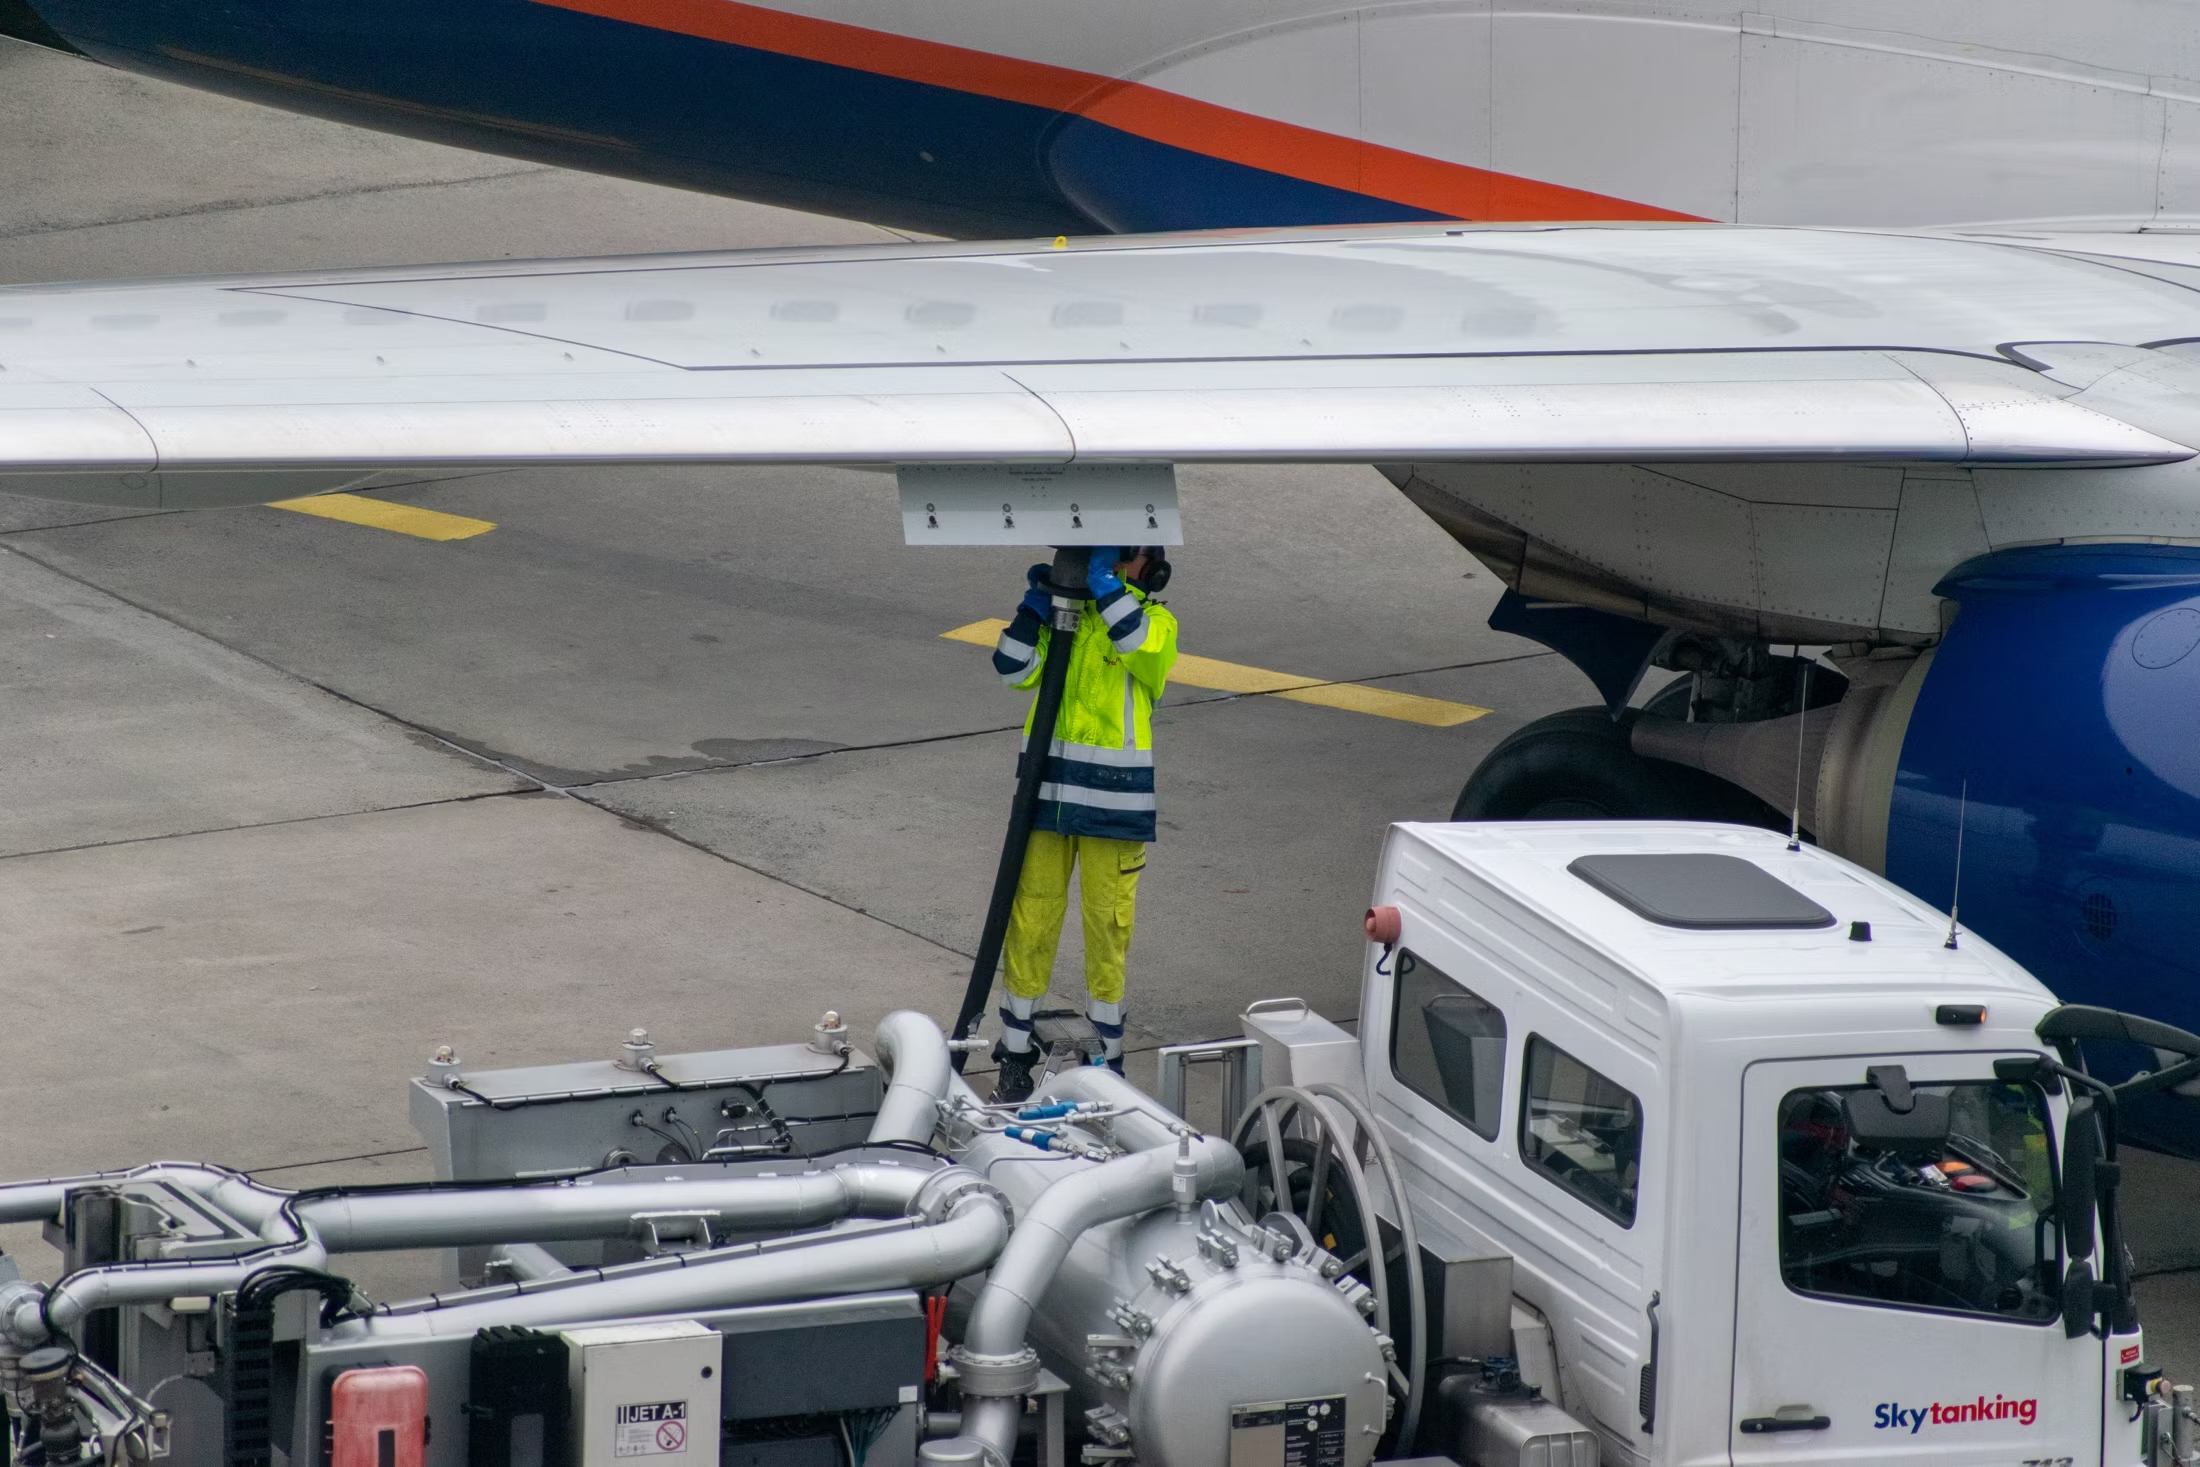
\includegraphics[width=0.5\textwidth]{figures/pressure-refuelling.jpeg}
    \caption{Pressure Refuelling of a Commercial Aircraft. Source: Tom Boon/Simple Flying}\label{fig:pressure-refuelling}
\end{figure}

The aviation industry is undergoing a significant transformation with the
advent of intelligent airports based on highly automated systems. Among these,
automated refuelling systems play a crucial role in ensuring efficient and
accurate refuelling of aircraft. However, one of the main challenges of this
automation process is the accurate detection of the aircraft's refuelling port,
which is relatively small and can easily be obscured by other visual elements
on or near an aircraft. Scanning the entire area of each video frame is both
time-consuming and inaccurate. It is therefore essential to develop a more
efficient and accurate method of locating the refuelling port.

This thesis aims to address this challenge by developing a new AI model that
uses the temporal relationships between successive frames of a video to predict
the location of the refuelling port in subsequent frames. By focusing the
analysis on the most relevant areas of the video sequence, this approach has
the potential to optimise both the speed and accuracy of the refuelling system.

Specific objectives of this thesis include conducting a comprehensive review of
state-of-the-art object detection and tracking methods, designing and
developing a real-time computer vision system capable of accurately detecting
and tracking the pressurised refuelling port of a commercial aircraft, the
implementation and evaluation of deep learning time series models for future
position prediction, the integration of Extended Kalman Filtering (EKF) into
deep learning models to improve the accuracy and robustness of future position
predictions, and the development of a real-time framework for predicting the
future position of the pressurised refuelling port.

By achieving these objectives, this thesis aims to make a significant
contribution to the development of intelligent airport systems and to improve
the efficiency and accuracy of automated refuelling systems at airports, while
reducing computing power requirements. The proposed framework has the potential
to be applied in various scenarios, such as different lighting conditions,
angles and orientations of refuelling ports, making it a versatile and
effective solution to the challenges of automated refuelling systems.
%%%%%%%%%%%%%%%%%%%%%%%%%%%%%%%%%%%%%%%%%%%%%%%%%%%%%%%%%%%%%%%%%%%%%%%%%%%%%%%%

%%%%%%%%%%%%%%%%%%%%%%%%%%%%%%%%%%%%%%%%%%%%%%%%%%%%%%%%%%%%%%%%%%%%%%%%%%%%%%%%
%%%%%%%%%%%%%%%%%%%%%%%%%%%%% LITERATURE REVIEW %%%%%%%%%%%%%%%%%%%%%%%%%%%%%%%%
\chapter{Literature Review}
\section{Automated Refulling Systems in the Aviation Industry}
Automated refueling systems have gained substantial importance in the aviation
industry due to their potential to enhance safety and efficiency. The concept
of Autonomous Aircraft Ground Refueling (AAGR) emerged in the 1980s, with
initial implementations featuring numbered markers near refueling ports to aid
in image processing and robotic automation~\cite{Schultz1986, Bennett1991,
    DatasetAGR}.

These systems streamline the refuelling process by using state-of-the-art
mechanisms and technologies to ensure accuracy and speed. A key element is the
pressurised fuel adaptor, which connects seamlessly to the aircraft
~\cite{HybridDatasetAGRV2}. Methods such as `PosEst' have been proposed to
capture and track objects in 3D, enabling the pressurised refuelling port to be
located precisely.~\cite{AGRPoseEstimation}.

In addition, autonomous in-flight refuelling technologies for Unmanned Aerial
Vehicles (UAV-AARs) have also been developed to extend their range, endurance
and payload capacity without significantly altering their original design. This
technology overcomes limitations in fuel capacity and endurance, enabling UAVs
to undertake longer missions~\cite{AARBinocularVision}.

The implementation of AAGR presents a number of challenges, including varying
lighting conditions, different refuelling port designs and potential
obstructions. Confidentiality issues associated with aircraft refuelling data,
as well as the lack of standardised workflows, also complicate the deployment
of advanced AAGR solutions, based on~\cite{DatasetAGR} data.

Accurately detecting and estimating the position of the fuelling adaptor is a
major hurdle. Current methods that rely on artificial features often encounter
occlusions and suffer from reduced reliability due to a low signal-to-noise
ratio, particularly over long distances~\cite{AGRPoseEstimation}. Variability
in lighting, weather conditions and the physical state of the refuelling
adapter further complicates detection and
localisation~\cite{HybridDatasetAGRV1}. Vision-based systems must operate in
real time and with minimal computational load, adding a new layer of
complexity.

The development of high-quality data sets for training and monitoring automated
refuelling systems is another major challenge. Collecting and processing these
datasets is often time-consuming and requires meticulous
configuration~\cite{HybridDatasetAGRV2}.

Visual measurement methods based on artificial features, such as spray marks or
LEDs, are commonly used in today's automated refuelling systems. The VisNav
system, developed by Valsek, uses light-emitting diodes emitting at different
frequencies to locate the centre of a beacon, employing a Gaussian least
squares differential correction algorithm to calculate the position of
the~\cite{AGRPoseEstimation} refuelling adaptor. Despite the advantages of
these methods, they remain sensitive to occlusion and low signal-to-noise
ratios at long distances.

Recent advances in Automatic Aircraft Ground Refuelling (AAGR) rely on computer
vision, artificial intelligence and robotics to achieve high levels of
automation. The integration of these technologies with Big Data has
significantly improved the feasibility and accuracy of AAGR systems thanks to
the creation of large datasets for training and validation. For example, an
Aircraft Ground Refuelling (AGR) dataset comprising more than 3,000 images from
13 databases was expanded to more than 26,000 images after augmentation,
enabling AGR scene recognition through image mining, augmentation and
classification~\cite{DatasetAGR}. In addition, recent innovations have
introduced hybrid datasets combining real and synthetic data for training and
validating~\cite{HybridDatasetAGRV1} systems. This approach offers a wide range
of scenarios and conditions, improving the robustness and accuracy of automated
refuelling systems.

Furthermore, in the field of autonomous aerial refuelling, current technologies
rely mainly on vision-based systems and sophisticated control algorithms. These
methods use a variety of sensors, including monocular and binocular cameras, to
detect and track drugs and refuelling probes.~\citet{AARCNN} demonstrated the
feasibility of real-time drug recognition and 3D localisation for autonomous
aerial drone refuelling using monocular computer vision. In
addition,~\citet{Chen2011} explored the application of 3D flash lidar for drug
tracking~\cite{AARCNN}. The probe and drogue refuelling system involves the
refuelling aircraft towing a refuelling hose with a drogue at the end, while
the pilot of the receiving aircraft manoeuvres to insert the probe into the
drogue. For unmanned aerial refuelling, this process is carried out
autonomously. Although DGPS offers high location accuracy, it faces challenges
such as lock-in problems and low bandwidth in air-to-air refuelling
applications~\cite{AAREKF}.
%%%%%%%%%%%%%%%%%%%%%%%%%%%%%%%%%%%%%%%%%%%%%%%%%%%%%%%%%%%%%%%%%%%%%%%%%%%%%%%%

\newpage
\section{Object Detection and Tracking in Computer Vision}
In Computer Vision, Object Detection refers to the identification and location
of individual objects within an image, providing both spatial information
(bounding boxes) and confidence scores, which represent the probability that
each detected object belongs to the predicted
class~\cite{huggingface2023objectdetection}. For example, in the following
image, there are five detections, including one `ball' with a confidence level
of 98\% and four `people' with confidence levels of 98\%, 95\%, 97\% and 97\%.

\begin{figure}[H]
    \centering
    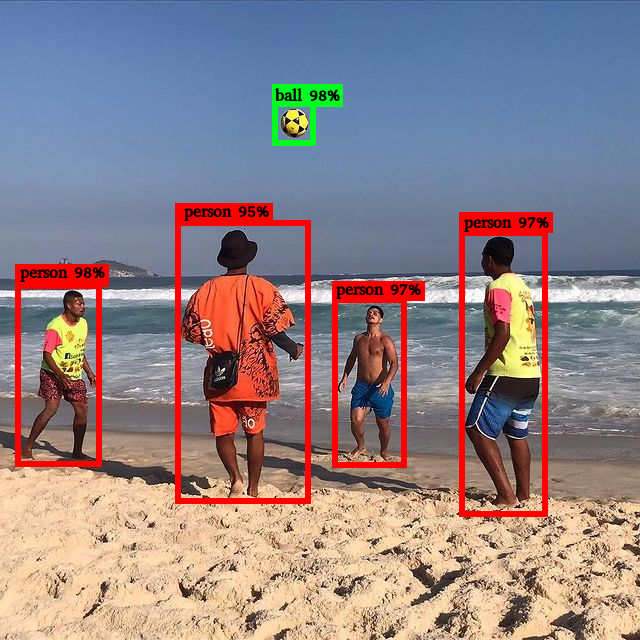
\includegraphics[width=0.3\textwidth]{figures/intro_object_detection.png}
    \caption{Example of outputs from an object detector~\cite{huggingface2023objectdetection}.}\label{fig:object-detection}
\end{figure}

Over the last few decades, Object Detection models based on Deep Learning have
enjoyed remarkable success. These models fall into two main categories:
two-stage detectors and single-stage detectors. 

On the one hand, two-stage detectors, such as
R-CNN~\cite{DBLP:journals/corr/GirshickDDM13}, Fast
R-CNN~\cite{DBLP:journals/corr/Girshick15}, Faster R-CNN~\cite{Ren2017} and
R-FCN~\cite{DBLP:journals/corr/DaiLHS16}, first generate region proposals and
then refine these proposals into precise anchor boxes. While these models excel
in detection accuracy, they typically suffer from large model sizes and slower
detection speeds~\cite{SurveyDLOD, ODNetworkUAVCNNTransformer}.

On the other hand, single-stage detectors, including the SSD (Single Shot
Multibox Detector)~\cite{DBLP:journals/corr/LiuAESR15}, YOLO (You Only Look
Once) series~\cite{DBLP:journals/corr/RedmonDGF15,
    DBLP:journals/corr/RedmonF16, DBLP:journals/corr/abs-2004-10934,
    chen2023yoloms, DBLP:journals/corr/abs-2107-08430, YOLOv5Release, li2023yolov6,
    YOLOv8, wang2024yolov9, xu2022ppyoloe, wang2023goldyolo, xu2023damoyolo,
    wang2024yolov10}, and RetinaNet~\cite{lin2018focal} directly predict object
locations and categories in a single network pass. These models are known for
their high detection speeds but sometimes compromise accuracy~\cite{SurveyDLOD,
    ODNetworkUAVCNNTransformer}.

\begin{figure}[H]
    \centering
    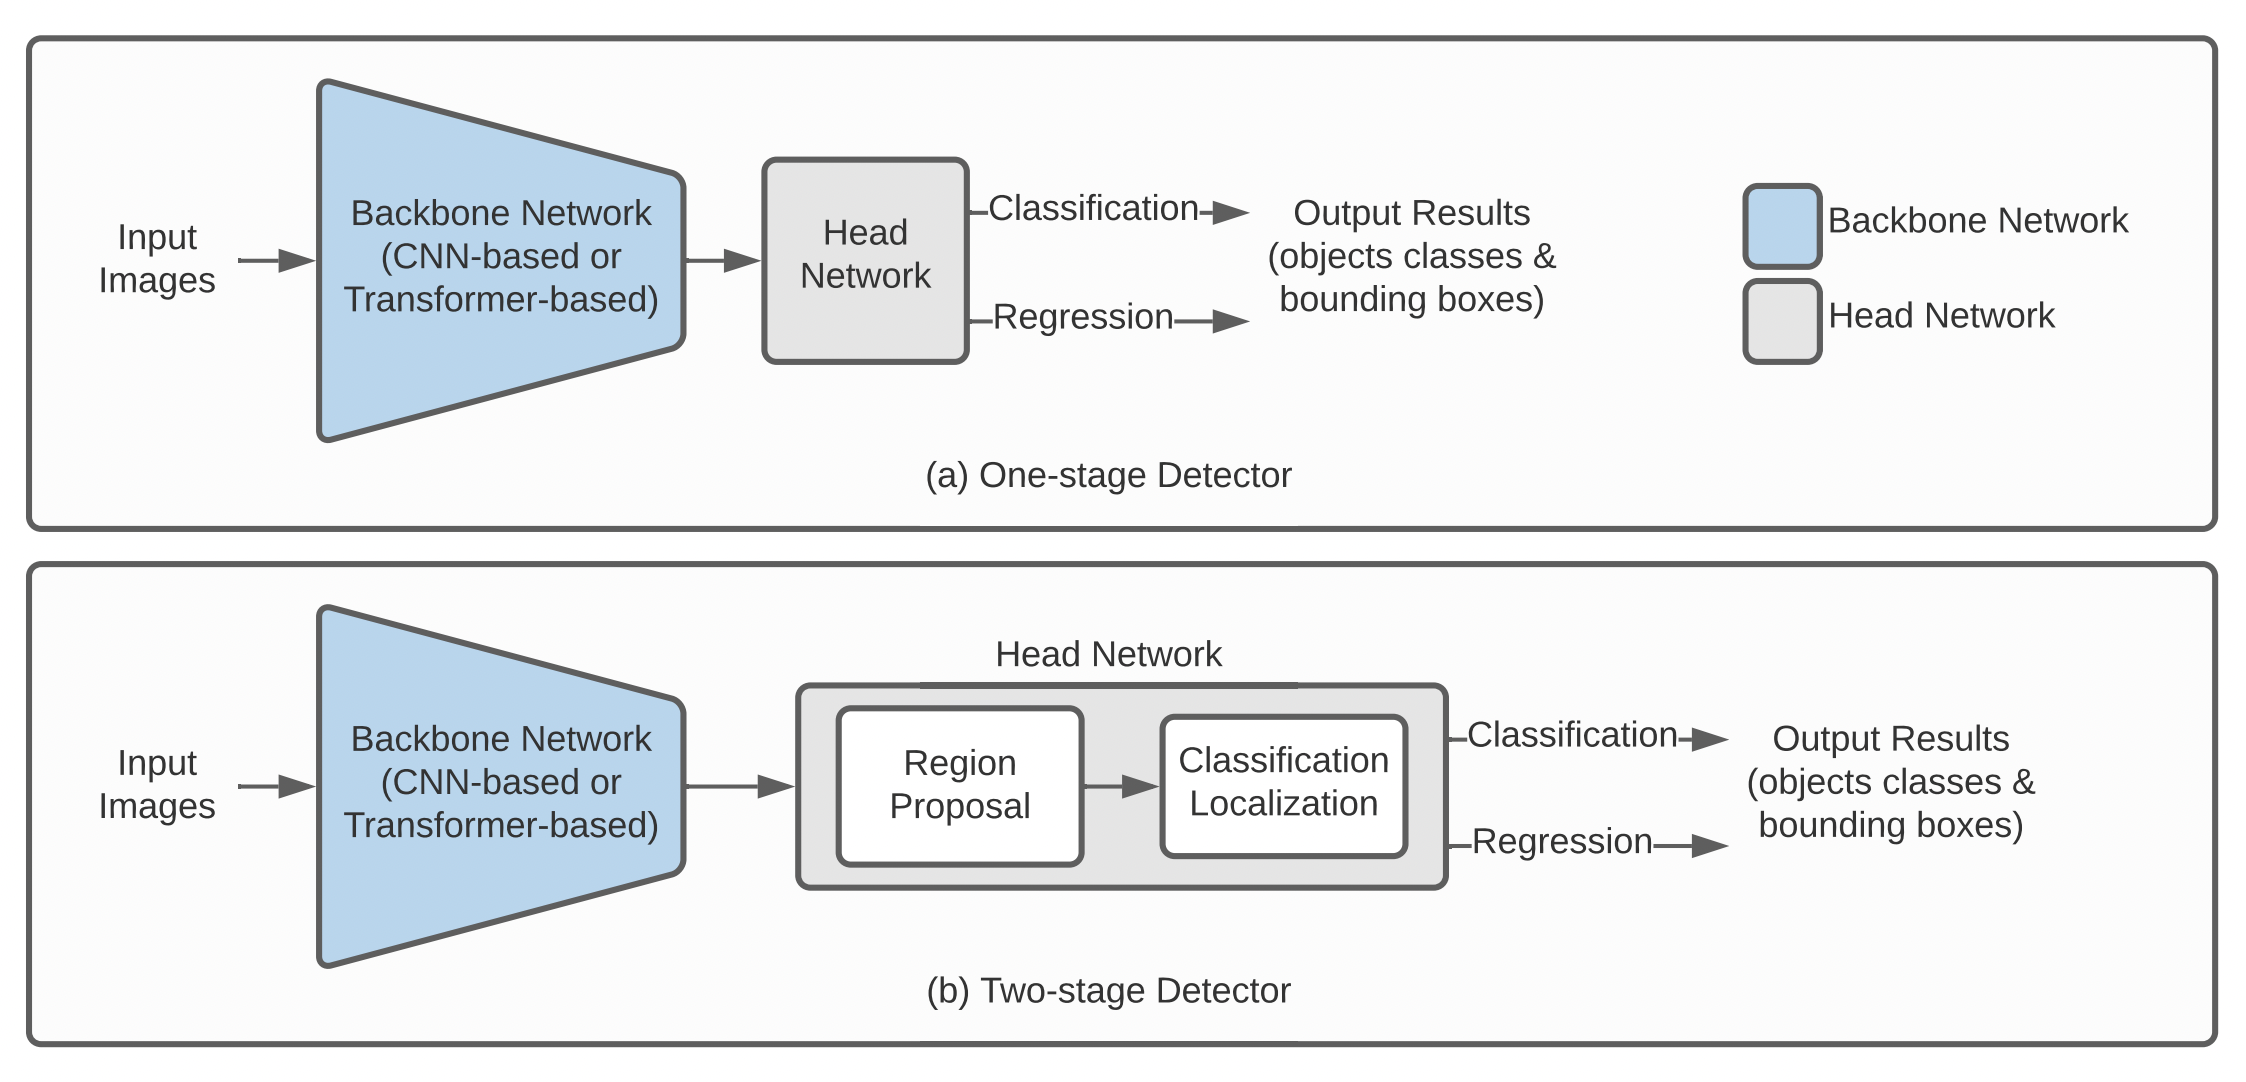
\includegraphics[width=0.8\textwidth]{figures/one-stage_two-stage_OD.png}
    \caption{Basic deep learning-based one-stage vs two-stage object detection model architectures~\cite{SurveyDLOD}.}\label{fig:two-stage-vs-single-stage}
\end{figure}

Evaluating Object Detection models involves several key metrics to measure
their performance. One common metric is Intersection over Union (IoU), which
measures the overlap between a predicted bounding box and a ground-truth
bounding box, as shown in Figure~\ref{fig:iou-metric}.

\begin{figure}[H]
    \centering
    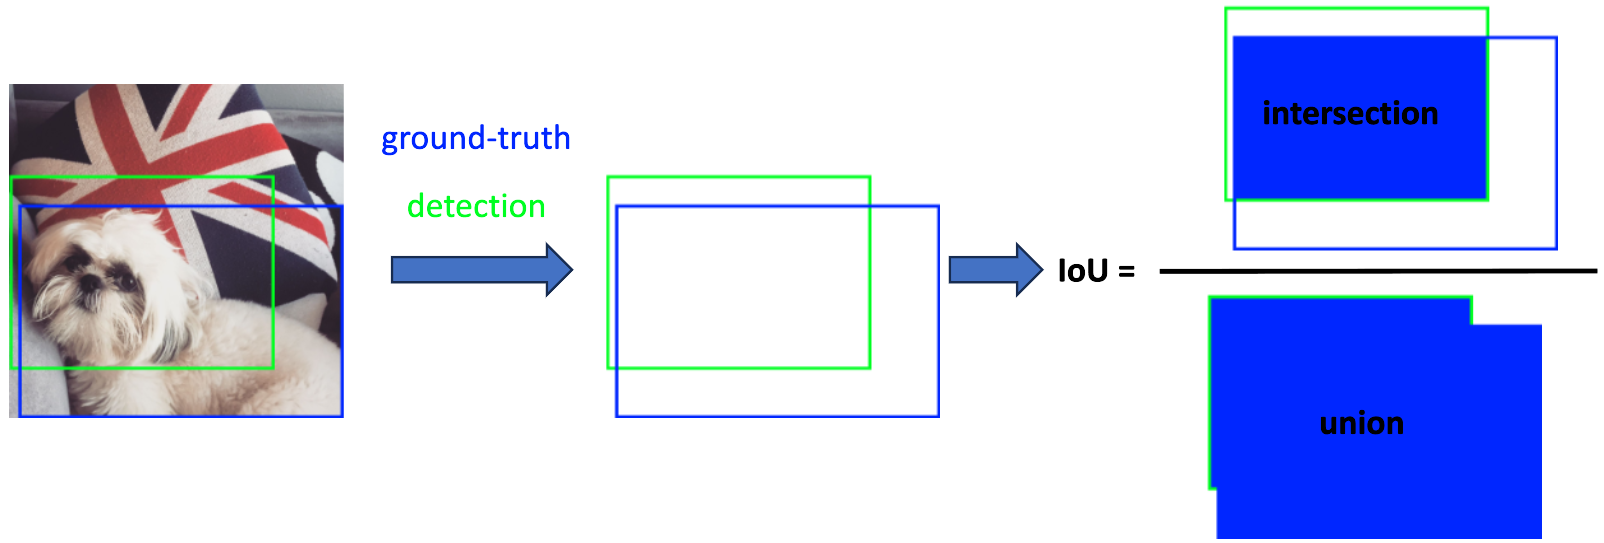
\includegraphics[width=0.8\textwidth]{figures/iou.png}
    \caption{Intersection over Union (IoU) between a detection (in green) and ground-truth (in blue).~\cite{huggingface2023objectdetection}}\label{fig:iou-metric}
\end{figure}

Based on the IoU metric, a detection can be classified as a \textbf{True
    Positive (TP)} or a \textbf{False Positive (FP)} depending on whether the IoU
value exceeds a certain threshold ($T_{IoU}$). If the IoU is above the
threshold, the detection is considered correct (TP); otherwise, it is
classified as a False Positive (FP). Additionally, \textbf{False Negatives
    (FN)} refer to ground truth objects not detected by the model, while
\textbf{True Negatives (TN)} are correctly classified background
detections~\cite{huggingface2023objectdetection}. These classifications allow
for the calculation of the following metrics:

\begin{itemize}
    \item \textbf{Precision}: The ratio of True Positives to the total number of
          detections, measuring the model's ability to avoid false positives:
          \begin{equation}
              \text{Precision} = \frac{\text{TP}}{\text{TP} + \text{FP}}
          \end{equation}

    \item \textbf{Recall}: The ratio of True Positives to the total number of ground-truth objects, measuring the model's ability to avoid false negatives:
          \begin{equation}
              \text{Recall} = \frac{\text{TP}}{\text{TP} + \text{FN}}
          \end{equation}
\end{itemize}

Common metrics used to evaluate Object Detection include:

\begin{itemize}
    \item \textbf{Average Precision (AP)}: This combines precision and recall, providing a single figure summarizing the model's performance across different confidence thresholds. Common versions are AP@.5 (with a threshold of 0.5 IoU) and AP@[.5:.05:.95], which calculates the average of AP values over several IoU thresholds~\cite{huggingface2023objectdetection}.
    \item \textbf{Average Recall (AR)}: This measures the recall of the model averaged across multiple IoU thresholds. It can be computed for different numbers of detections per image, such as AR@1, AR@10, etc.~\cite{huggingface2023objectdetection}.
    \item \textbf{Inference Time}: The time taken by the model to process an image, which is critical for applications requiring real-time detection~\cite{huggingface2023objectdetection}.
    \item \textbf{Model Size}: The number of parameters or the size of the model, affecting deployment, especially on devices with limited resources~\cite{huggingface2023objectdetection}.
    \item \textbf{Efficiency}: This considers the trade-off between accuracy and speed, often visualized using the AP vs. inference time curve~\cite{huggingface2023objectdetection}.
\end{itemize}

In addition to Object Detection, Object Tracking is another critical task in
Computer Vision, involving the continuous monitoring of objects across video
frames. Object Tracking methods can be broadly classified into two categories:
\textbf{Generative Trackers} and \textbf{Discriminative
    Trackers}~\cite{SurveyVisualOT}. Generative trackers are capable of handling
challenging scenarios such as occlusion and large-scale variation through
particle sampling strategies, often integrated with various appearance models,
including sparse representation and energy of motion. Discriminative trackers,
by contrast, build robust classifiers using hand-crafted or deep
features~\cite{SurveyVisualOT}. The combination of generative and
discriminative approaches, as well as the integration of deep learning
techniques such as fully revolutionary networks and Transformer models, has led
to significant improvements in object detection
performance~\cite{OverviewCorrelationAlgoOT, SuveyAdvancesSingleOTMethods,
    SurveyModernODModels}. In addition, the speed and computational requirements of
these algorithms are critical factors influencing their practical
applicability~\cite{SuveyAdvancesSingleOTMethods, SurveyModernODModels,
    SurveyTransformersSingleOT}. Advanced techniques in object tracking leverage
both generative and discriminative models to amplify tracking efficacy. The
utilisation of deep trackers has evidenced superior results on public tracking
datasets, attributed to their potent feature extractors, accurate bounding box
regressors, and discriminative classifiers~\cite{SurveyTransformersSingleOT}.
Techniques such as deformable convolution and Transformer models extend
traditional convolution or correlation methodologies to execute global feature
matching, thereby enhancing tracking accuracy. The incorporation of contextual
or knowledge information can substantially elevate performance, with
methodologies like Particle Filtering, also recognised as Sequential Monte
Carlo (SMC) methods, framed as problems of Bayesian inference in state
space~\cite{SurveySmallObjectDetection, SmallObjectDetectionPositonPrediction}.
The extended Kalman Filtering (EKF) is another advanced technique that has been
employed to improve tracking accuracy by predicting the current status through
the previous status and modifying the prediction result based on observation
information~\cite{SuveyAdvancesSingleOTMethods, SurveyModernODModels}. Despite
these advancements, the integration of these methods in a complementary manner
remains an open research area with substantial potential for advancing the
field~\cite{OverviewCorrelationAlgoOT, SuveyAdvancesSingleOTMethods}.

\section{Deep Learning for Spacio-Temporal Prediction}
Time series prediction involves processing sequential data to predict future
events or values. Various deep learning models have been applied to this task,
requiring several preparatory steps such as collecting data, designating
attribute types, dealing with inconsistencies and storing datasets. These
datasets are usually classified into units of time such as seconds, minutes and
hours, allowing the construction of metadata for machine
learning~\cite{FFPSpaceSystemVehicles}.

\subsection*{Early Approaches and Models}
The problem of predicting the future locations of objects has been extensively
studied, particularly for static surveillance cameras. Initial efforts utilised
recurrent neural networks (RNNs), including long-term memory networks (LSTMs)
and gated recurrent units (GRUs), in an encoder-decoder format to encode past
observations and decode future locations. Early models integrated additional
inputs such as environmental data and semantic actions to enhance prediction
accuracy. For instance,~\citet{Alahi2016} proposed a Social-LSTM to model
pedestrian trajectories and interactions, further improving global context
capture through a social pooling module~\cite{FusionGRU}. Recent advancements
have leveraged generative models and attention mechanisms to manage complex
scenes involving multiple interacting agents~\cite{FusionGRU}.

\subsection*{Frame-Based Approaches in Spatio-Temporal Prediction}

Video prediction, a critical task in spatio-temporal data analysis, involves
forecasting future frames based on past and current frames. This process
requires understanding both spatial and temporal dynamics within the data.

\subsubsection*{Convolutional LSTM (ConvLSTM)}

ConvLSTM integrates convolutional operations into LSTM units to better capture
spatial features in addition to temporal dependencies~\cite{ConvLSTM}. By
processing video data as sequences of frames, ConvLSTM effectively models the
spatio-temporal dependencies necessary for accurate video prediction. Each
frame serves as a spatial unit, and the sequence of frames provides temporal
context, allowing the model to predict future frames by learning from the
patterns in previous ones.

\subsubsection*{Cubic LSTM for Video Prediction}

The Cubic Long Short-Term Memory (CubicLSTM) unit, as proposed
by~\citet{CubicLSTMsVideoPrediction}, extends the capabilities of ConvLSTM by
separately processing spatial and temporal information through three branches:
temporal, spatial, and output. This approach mitigates the computational burden
and enhances prediction accuracy. Specifically:
\begin{itemize}
    \item The \textit{temporal branch} processes motion information by analysing the
          sequence of frames over time.
    \item The \textit{spatial branch} captures object information within individual
          frames.
    \item The \textit{output branch} combines temporal and spatial information to
          generate predicted future frames.
\end{itemize}
This separation of concerns allows the model to handle the complexities of video data more effectively, resulting in more accurate predictions of future frames.

\subsubsection*{Dual-Branch Spatial-Temporal Learning Network}

Huang and Guan~\cite{DualBranchSpatialTemporalLearningNetworkVideoPrediction}
proposed a dual-branch video prediction network that aims to generate
high-quality future frames by simultaneously capturing complex motion patterns
and preserving appearance information. Their network includes two distinct
units:
\begin{itemize}
    \item The \textit{motion prediction unit (MPU)} focuses on inter-frame motion and
          intra-frame appearance by using depth and multiple-scale convolutions, along
          with temporal attention mechanisms to enhance feature interactions over time.
    \item The \textit{spatial prediction unit (SPU)} concentrates on spatial information,
          ensuring appearance consistency across video frames by capturing various
          appearance features.
\end{itemize}
This dual-branch approach addresses the limitations of relying on external information or complex state transition units, resulting in better visual quality and fewer blurry artifacts in predicted frames.

\subsubsection*{Unsupervised Video Forecasting with Flow Parsing}
\citet{UnsupervisedVideoForecastingFlowParsingMechanism} introduced an unsupervised video forecasting approach that incorporates a flow parsing mechanism. This model separates the motion and appearance learning processes:
\begin{itemize}
    \item The \textit{motion stream} predicts optical flow between frames to capture
          dynamic changes.
    \item The \textit{appearance stream} reconstructs frames to preserve spatial details.
\end{itemize}
By integrating these streams, the model can predict future frames with improved motion accuracy and appearance fidelity.

\subsubsection*{Joint Optimization with Synthesis and Optical Flow Estimation}
\citet{VideoFramePredictionByJointOptimizationWithSynthesisAndOpticalFlowEstimation}
proposed a method that jointly optimizes frame synthesis and optical flow
estimation. Their approach leverages:
\begin{itemize}
    \item A \textit{frame synthesis network} to generate predicted frames.
    \item An \textit{optical flow estimation network} to capture motion dynamics between
          frames.
\end{itemize}
This joint optimization enhances the model's ability to produce accurate and visually coherent future frames.

\subsubsection*{Predicting Future Frames for Fast-Moving Objects with Motion Blur}

\citet{Lee2020} addressed the challenge of predicting future frames
for fast-moving objects, which often result in motion blur. Their model
includes:
\begin{itemize}
    \item A \textit{motion deblurring module} to reduce blur effects in fast-moving
          scenes.
    \item A \textit{future frame prediction module} that leverages the deblurred frames
          to enhance prediction accuracy.
\end{itemize}
This approach ensures that the predicted frames maintain high visual quality even in challenging conditions.

\subsection*{Applications and Case Studies}

In various applications, the frame-based approach to spatio-temporal prediction
has proven highly effective:

\subsubsection*{Moving-MNIST Dataset}

The Moving-MNIST dataset consists of sequences of moving handwritten digits.
Each sequence includes a series of frames, and the goal is to predict future
frames based on the observed ones. The CubicLSTM-based CubicRNN demonstrated
superior accuracy compared to traditional ConvLSTM models, showcasing its
ability to capture both motion and spatial features
effectively~\cite{DBLP:journals/corr/SrivastavaMS15,
    CubicLSTMsVideoPrediction}.

\begin{figure}[H]
    \centering
    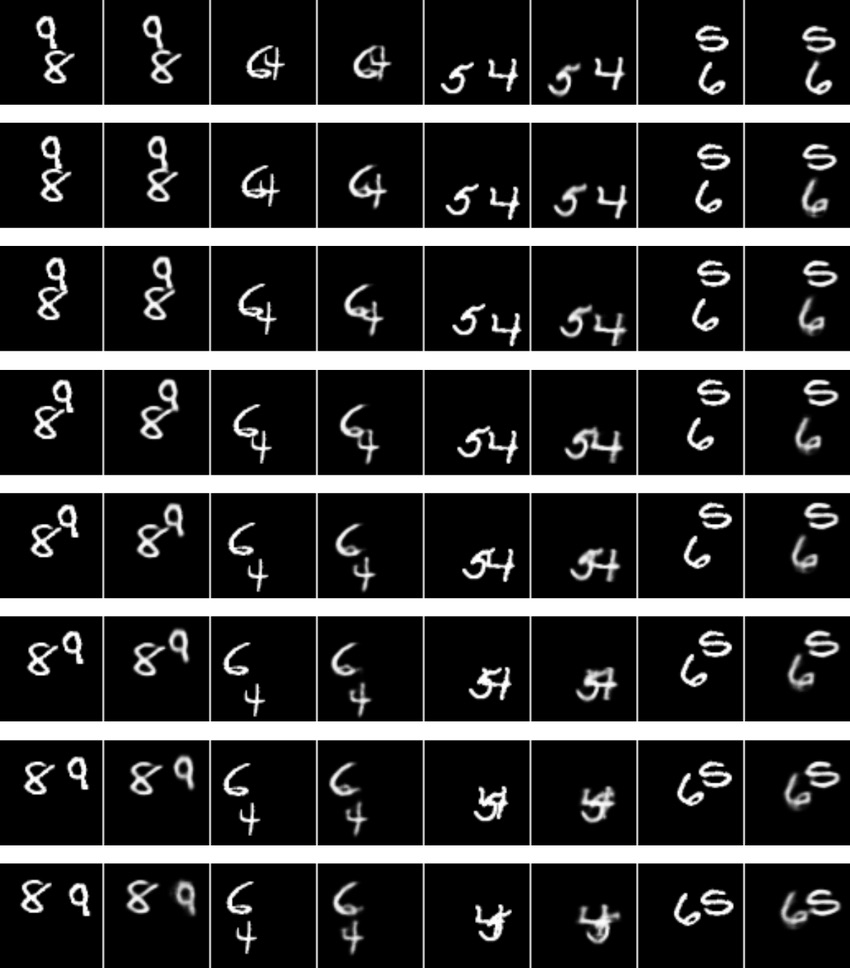
\includegraphics[width=0.3\textwidth]{figures/2-digit-Moving-MNIST-data-Fig-5-3-digit-Moving-MNIST-data.jpeg}
    \caption{2-digit Moving MNIST data~\cite{DBLP:journals/corr/SrivastavaMS15}}\label{fig:moving-mnist}
\end{figure}

\subsubsection*{Robotic Pushing Dataset}

This dataset involves sequences of robotic arms pushing objects, with each
frame representing a step in the sequence. The CubicLSTM model, combined with
convolutional dynamic neural advection (CDNA) models, achieved higher accuracy
and generated clearer frames compared to ConvLSTM and CNN-based models. This
application highlights the importance of accurately predicting future frames to
understand and anticipate the movements of robotic
systems~\cite{DBLP:journals/corr/FinnGL16, CubicLSTMsVideoPrediction}.

\subsubsection*{KTH Action Dataset}

The KTH Action dataset features videos of people performing various actions,
with each video divided into frames. The CubicLSTM model provided more accurate
and visually consistent predictions of future frames compared to other
state-of-the-art models like DrNet and MCnet. This demonstrates the model's
effectiveness in understanding and predicting human actions over
time~\cite{KTH, CubicLSTMsVideoPrediction}.

\subsubsection*{UCF Sports Dataset}

Huang and Guan's dual-branch network was tested on the UCF Sports dataset,
which includes complex motion patterns and large movements. Their method
outperformed other state-of-the-art methods in terms of visual quality and
motion accuracy, as evidenced by superior metrics such as PSNR, SSIM, and
LPIPS. The results validate the network's ability to handle intricate video
prediction tasks without relying on additional information~\cite{UCFSport,
    DualBranchSpatialTemporalLearningNetworkVideoPrediction}.

\subsection*{Transformer Models for Frame-Based Prediction}

Transformer model, introduced by~\citet{Vaswani2017}, has revolutionised
sequence modeling with its efficient and powerful network structure. For video
prediction, transformers leverage self-attention mechanisms to capture
long-range dependencies across frames. The~\citet{HowDoUGoWhere} study shows
how transformers can effectively learn mobility patterns from historical frame
sequences, achieving state-of-the-art performance in next-location prediction
tasks.

\subsection*{Validation and Efficacy}

Extensive experiments and validations on real-world datasets have affirmed the
efficacy of frame-based models like ConvLSTM, CubicLSTM, and the dual-branch
network in improving prediction accuracy. The work
of~\citet{SpatioTemporalTransformerRecommender} discusses the application of
transformers and self-attention mechanisms in sequence prediction, highlighting
their effectiveness in various contexts. These models demonstrate the
importance of frames as fundamental units of analysis in spatio-temporal
prediction tasks.

By leveraging deep learning techniques, especially advanced models like
CubicLSTM, dual-branch networks, and transformers, the accuracy and efficiency
of spatio-temporal predictions can be significantly enhanced, contributing to
improved outcomes in various real-world applications.

%% Back matter
%
% This is where we include references and appendices

\bibliographystyle{abbrvnat}
\bibliography{LaTeX,CUCitations}

\appendix
\chapter{Ethical Approval Letter}
Insert your Ethical Approval Letter as the first appendix.

\chapter{Extra Data}
This is a sample of thesis text. This is a sample of thesis text. This is a
sample of thesis text. This is a sample of thesis text. This is a sample of
thesis text.

This is a sample of thesis text. This is a sample of thesis text. This is a
sample of thesis text. This is a sample of thesis text. This is a sample of
thesis text.

\end{document}

